% coding:utf-8

%FOSAET, a LaTeX-Code for a electrical summary of basic electronics
%Copyright (C) 2013, Daniel Winz, Ervin Mazlagic

%This program is free software; you can redistribute it and/or
%modify it under the terms of the GNU General Public License
%as published by the Free Software Foundation; either version 2
%of the License, or (at your option) any later version.

%This program is distributed in the hope that it will be useful,
%but WITHOUT ANY WARRANTY; without even the implied warranty of
%MERCHANTABILITY or FITNESS FOR A PARTICULAR PURPOSE.  See the
%GNU General Public License for more details.
%----------------------------------------

\subsection{Aktiver Tiefpass 2. Ordnung}
\label{filt:o2-tp}
\begin{figure}[h!]
	\centering
	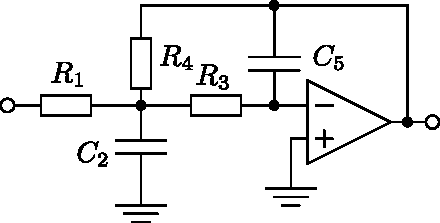
\includegraphics[scale=\schscale]{op_tp_o2.pdf}
	\caption{Aktiver Tiefpass 2. Ordnung}
	\label{sch:op-tp-o2}
\end{figure}
\[ \frac{-H \cdot {\omega_0}^2}
{s^2 + \alpha \cdot \omega_0 \cdot s + {\omega_0}^2} \]
\[ \frac{V_{out}}{V_{in}} 
= \frac{-H \cdot \frac{1}{R_3 \cdot R_4 \cdot C_2 \cdot C_5}}
{s^2 + s \cdot \frac{1}{C_2} 
\left(\frac{1}{R_1} + \frac{1}{R_3} + \frac{1}{R_4}\right) 
+ \frac{1}{R_3 \cdot R_4 \cdot C_2 \cdot C_5}} \]
\[ \alpha = \frac{1}{Q} \]

\subsubsection{Dimensionierung}
\[ C_5 \text{ wählen} \]
\[ k = 2 \pi \cdot f_0 \cdot C_5 \]
\[ C_2 = \frac{4}{\alpha^2} (H + 1) \cdot C_5 
= 4 \cdot Q^2 (H + 1) \cdot C_5 \]
\[ R_1 = \frac{\alpha}{2 \cdot H \cdot k} 
= \frac{1}{2 \cdot Q \cdot H \cdot k} \]
\[ R_3 = \frac{\alpha}{2 \cdot (H + 1) \cdot k} 
= \frac{1}{2 \cdot Q \cdot (H + 1) \cdot k} \]
\[ R_4 = \frac{\alpha}{2 \cdot k} = \frac{1}{2 \cdot Q \cdot k} \]
